\graphicspath{{./Images/Kapitel4/}}

\section{Bussysteme}

\subsection{Automotive Ethernet}
\subsubsection{Anwendung}
Für Ethernet im Automotive Bereich wird der Standard IEEE 802.3 verwendet. Trotz seiner hohen Beliebtheit und Verbreitung war Ethernet im Automotive Bereich lange Zeit undenkbar, vor allem da es keine Echtzeit erfüllen kann und für kleine Anwendungen zu teuer ist. Moderne Anwendungen (z.B. komplexere Assistenzsysteme, Diagnose- oder Multimedia-Anwendungen) fordern jedoch immer höhere Datenraten, so dass Ethernet immer mehr Beachtung bekommt. Es wurden auch Protokolle und Technologien entwickelt, um Ethernet besser an die Anforderungen anzupassen. Es gibt mit TimeTriggeredEthernet/SAE AS6802 einen echtzeitfähigen Ethernet Bus und durch Audio-Video-Bridging können komplexere Multi-Media-Anwendungen, z.B. Surround Sound oder synchrone Wiedergabe von Audio/Video-Dateien, realisiert werden. Um Kosten und Leitungen zu sparen wurde 100Base-T1 entwickelt, hier wird nur ein verdrillter Kupferdraht benutzt. \cite{.MH_Ethernet}

\subsubsection{Topologie}
Ethernet wird im Automotive Bereich oft in der Stern- (siehe Abbildung \ref{fig:stern}), Bus- (siehe Abbildung \ref{fig:bus}) oder Baumtopologie (siehe Abbildung \ref{fig:baum}) verwendet. Dies ist ein neuer Ansatz, da die meisten bisherigen Bussysteme nahezu nur auf die Stern- und Bustopologie setzen.

\cite{.MH_Vehicle}

\begin{figure}[h!]
	\centering
	\begin{subfigure}[b]{0.4\textwidth}
		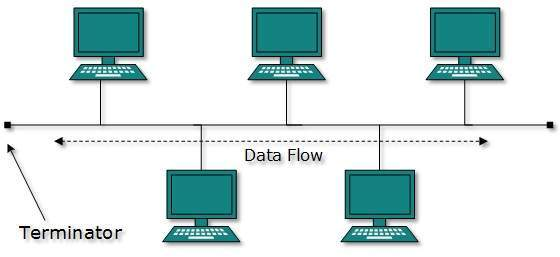
\includegraphics[width=\linewidth]{bus-topology.jpg}
		\subcaption[2.bp.blogspot.com/-R-uihxzRU6g/WOIFGLjqtMI/AAAAAAAAEdg/X3YgTGUxQ8MSCbm14OsABMnhWUTK-Ee-gCLcB/s1600/bus\textunderscore topology.jpg]{Bus}
		\label{fig:bus}
	\end{subfigure}
	\begin{subfigure}[b]{0.4\textwidth}
		\includegraphics[width=\linewidth]{stern-topology.jpg}
		\subcaption[slideplayer.org/slide/791365/2/images/3/Sternstruktur+(Ethernet+Twisted+Pair).jpg]{Stern}
		\label{fig:stern}
	\end{subfigure}
	\begin{subfigure}[b]{0.4\textwidth}
		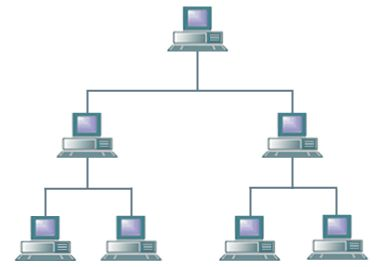
\includegraphics[width=\linewidth]{tree-topology.jpg}
		\subcaption[units.folder101.com/cisco/sem1/Notes/ch2-topologies/tree.gif]{Baum}
		\label{fig:baum}
	\end{subfigure}
	\caption{Ethernet Topologie}
\end{figure}

\subsubsection{Vor- und Nachteile}
\begin{tabular}{l|l}
	\textbf{Vorteile} & \textbf{Nachteile}\\
	\hline hohe Datenrate & hohe Kosten\\
	\hline neue Technologien z.B. Service discovery,  & keine Echtzeitfähigkeit, nicht\\
	DNS oder Streams für Multimedia & deterministisch\\
	\hline leichte Anbindung für IOT und Internet & Umdenken/Umdesignen für neue \\
	& Topologie und neuen Ansatz\\
	\hline viele Standardimplementationen und&\\
	Wiederverwertbarkeit der Software&\\
	\hline einfacher Austausch von Komponenten &\\
\end{tabular}

\subsection{MOST}		
\subsubsection{Anwendung}
Der MOST-Bus (Media Oriented Systems Transport) wird von der MOST Cooperation standardisiert und wird im Automotive Bereich nahezu ausschließlich für Multi-Media-Anwendungen eingesetzt. Durch seine hohe Datenrate kann es schnell viele Daten zwischen den Komponenten verschicken.


\cite{.MH_Vehicle}

\subsubsection{Topologie}
Ein MOST-Netzwerk ist immer als synchronisierter Ring aufgebaut (siehe Abbildung \ref{fig:ring}). Es gibt immer einen Master, der die Synchronisation steuert. Alle Komponenten haben eine Kontrollkanal, auf der Daten zum Status des Systems/Netzwerks gesendet werden. Zudem gibt es mehrere synchrone und asynchrone Kanäle, die sich die Bandbreite, je nach Last, teilen.
Auf dem synchronen Kanälen werden fortlaufende Daten, z.B. Audio- oder Videostreams verschickt.
Die asynchronen Kanäle sind für Daten reserviert, die nicht fortlaufend entstehen, aber schnell verarbeitet werden sollen. Z.B. Nutzereingaben zum Überspringen eines Songs oder Eingabe ins Navi. \cite{BP01}

\begin{figure}[h!]
	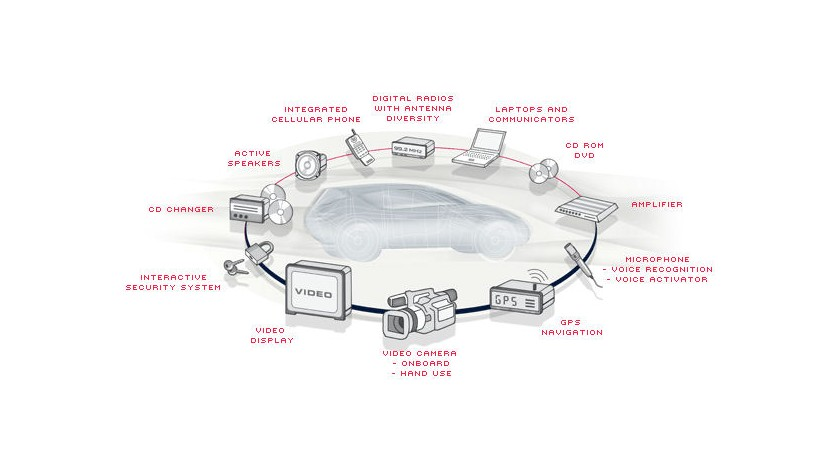
\includegraphics[width=\linewidth]{most-ring.jpg}
	%\caption[https://images.tecchannel.de/bdb/361603/840x473.jpg]{MOST Ring}
	\label{fig:ring}
\end{figure}

\subsubsection{Vor- und Nachteile}
\begin{tabular}{l|l}
	\textbf{Vorteile} & \textbf{Nachteile}\\
	\hline hohe Datenrate & hohe Kosten\\
	\hline einfacher Austausch von Komponenten & proprietäre Hardware\\
	\hline einheitliche Schnittstellen von Komponenten &\\
\end{tabular}

\subsection{Bluetooth}		
\subsubsection{Anwendung}
Bluetooth wird durch die Bluetooth Special Interest Group, ein Verband aus derzeit über 2000 Unternehmen,  standardisiert. Momentan ist Bluetooth 5 die aktuellste Version. Es wird im Automotive Bereich verwendet, um kostengünstige und kabellose Verbindungen aufzubauen. Der größte Bereich sind hierbei Multi-Media-Anwendungen, um beispielsweise Smartphones oder Kopfhörer anzubinden. \cite{BP01}

\subsubsection{Topologie}
Bluetooth Netzwerke haben immer einen Master, der die Kommunikation steuert. Dieser ist jedoch nicht fest, sondern wird erst beim Verbindungsaufbau ausgemacht.
Bluetooth-Netzwerke können entweder als Pico- oder Scatternet aufgebaut sein (siehe Abbildung \ref{fig:pico}).
                                                                                  
Ein Piconet ist eine Ansammlung von mindestens zwei Bluetooth-Geräten. Eines der Geräte übernimmt die Rolle des Masters und steuert die Kommunikation mit allen Slaves. Slaves können nur mit dem Master kommunizieren.

Ein Scatternet ist ein Zusammenschluss von mehreren Piconets, bei dem jeweils ein Knoten teil eines anderen Piconets ist. Dieser geteilte Knoten kann nicht gleichzeitig in beiden Netzen sein, sondern muss immer zwischen den Netzen wechseln. Der geteilte Knoten kann Master höchstens für eines der Netze sein.

\begin{figure}[h!]
	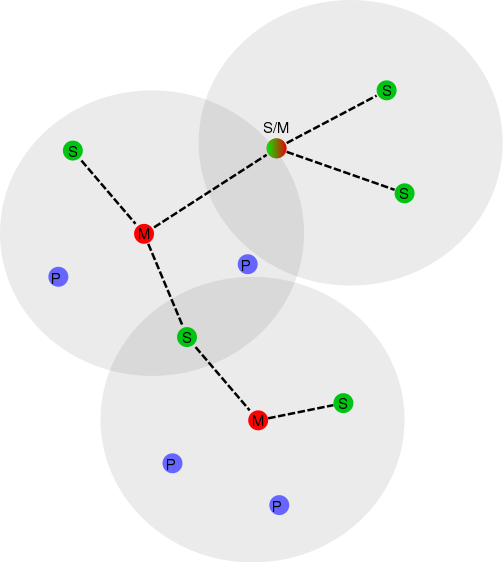
\includegraphics[width=0.7\linewidth]{pico-scatternet.png}
	%\caption[https://de.wikipedia.org/wiki/Scatternet#/media/Datei:BluetoothScatternet-de.svg]{Abbildung 4.5}
	\label{fig:pico}
\end{figure}

\subsubsection{Vor- und Nachteile}
\begin{tabular}{l|l}
	\textbf{Vorteile} & \textbf{Nachteile}\\
	\hline geringe Kosten & geringe Datenrate\\
	\hline kabellos & geringe Reichweite\\
	\hline Standardsoftware & störanfälliger als physische Busse\\
\end{tabular}

